\chapter{Problem Statement}
The thesis will focus on parliamentary proceedings from the German
\emph{Bundestag}. These proceedings are available online as PDF files dating
back to 1949, and have used essentially the same document layout and conventions
since the start. Semantically, the layout of these documents forms a shallow
tree:
\begin{center}
  \begin{forest}
    [root
      [topic
        [speech]
        [\dots]
        [speech]
      ]
      [\dots]
      [topic
        [speech]
        [\dots]
        [speech]
      ]
    ]
  \end{forest}
\end{center}
Each document consists of a series of topics to discuss, where each topic
contains a series of speeches made by the present politicians. The task to be
solved is retrieving these speeches as accurately and robustly as possible. Due
to the shallow nature of the document's layout, marking where a new speech
begins is sufficient for retrieving the layout to a sufficient degree. Although
this discards information about the overarching topics, this information is both
more difficult to extract (it is represented in a somewhat more free-form manner
in the text) and less fundamental to what the dataset might end up being used
for. Luckily, in this case a rule-based system for segmenting the files already
exists and was used to create a fairly large training set. Since in general such
a system will not exist and annotating the data by hand is expensive, a big
focus is on limiting the amount of required training data as much as possible;
it would be preferable if the system was able to learn sufficiently from a
handful (say, less than 5) of hand-annotated files.

\section{Dataset}
PDF files are unfortunately rather difficult to work with; being a vector-based
format, they have no internal concept of words or sentences. All that's
available are instructions for drawing a certain character at a certain
position. This means that even something as seemingly trivial as obtaining the
lines of text from a PDF requires some fairly involved logic and heuristics (for
instance, one would think that simply taking all characters on a page with the
same $y$ coordinate would be sufficient until realising that many documents have
a layout with two columns of text). This is dealt with by using the
\texttt{pdftohtml} script from the Poppler PDF rendering
library\footnote{https://poppler.freedesktop.org/}. This script converts a PDF
file to an XML file containing logical lines of text along with the coordinates
and size of the line. Figure~\ref{fig:example} shows an example of a portion of
a PDF file and the corresponding XML produced by \texttt{pdftohtml}.

\begin{figure}[htbp]
  \centering
  \begin{subfigure}[b]{0.6\textwidth} 
    \centering
    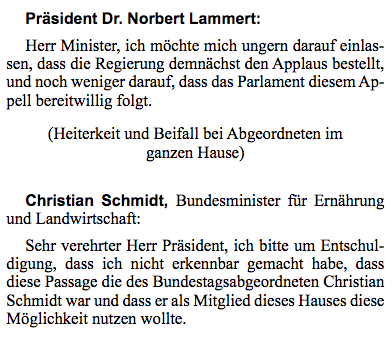
\includegraphics[width=\textwidth]{figures/source.png}
    \caption{The source PDF}
  \end{subfigure}
  \begin{subfigure}[b]{\textwidth}
	\centering
    \begin{lstlisting}[language=xml, morekeywords={text}]
      <text top="122" left="125" width="143" height="16" font="3">
          <b>Dr. Norbert Lammert </b>
      </text>
      <text top="122" left="269" width="83" height="17" font="4">
          (CDU/CSU):
      </text>
      <text top="142" left="125" width="328" height="17" font="4">
          Herr Alterspräsident, lieber Kollege Riesenhuber, ich
      </text>
      <text top="158" left="108" width="156" height="17" font="4">
          nehme die Wahl gerne an.
      </text>
      <text top="186" left="141" width="278" height="17" font="4">
          (Beifall im ganzen Hause – Abgeordnete aller
      </text>
      <text top="203" left="158" width="242" height="17" font="4">
          Fraktionen gratulieren dem Präsidenten)
      </text>
    \end{lstlisting}
    \caption{XML}
  \end{subfigure}
  \caption{The data representations}
  \label{fig:example}
\end{figure}

The dataset was obtained through a rule-based system as described in the
introduction, which annotates each \texttt{<text>} element of the XML files
with a boolean flag indicating whether said element starts a new speech. The
system was run on documents from the 18th electoral period of the
\emph{Bundestag}, consisting of 211 documents dating from 2013 to 2017. Together
these documents contain 43,252 \texttt{<text>} elements indicating the start of
speeches (that is, positive training samples), and 2,602,793 other elements
(negative samples). This adds to a total of 2,646,045 training samples, taking
up 503 MiB. This is a rather lopsided distribution (there are roughly 60
negative samples for each positive sample), which might have to be accounted for
by, for instance, subsampling negative samples before training.
Figure~\ref{fig:data_dist} shows the distribution of the number of positive
samples per file, giving a guideline as to how many files would have to be
annotated to reach a desired amount of positive samples.

\begin{figure}[htbp]
  \centering
  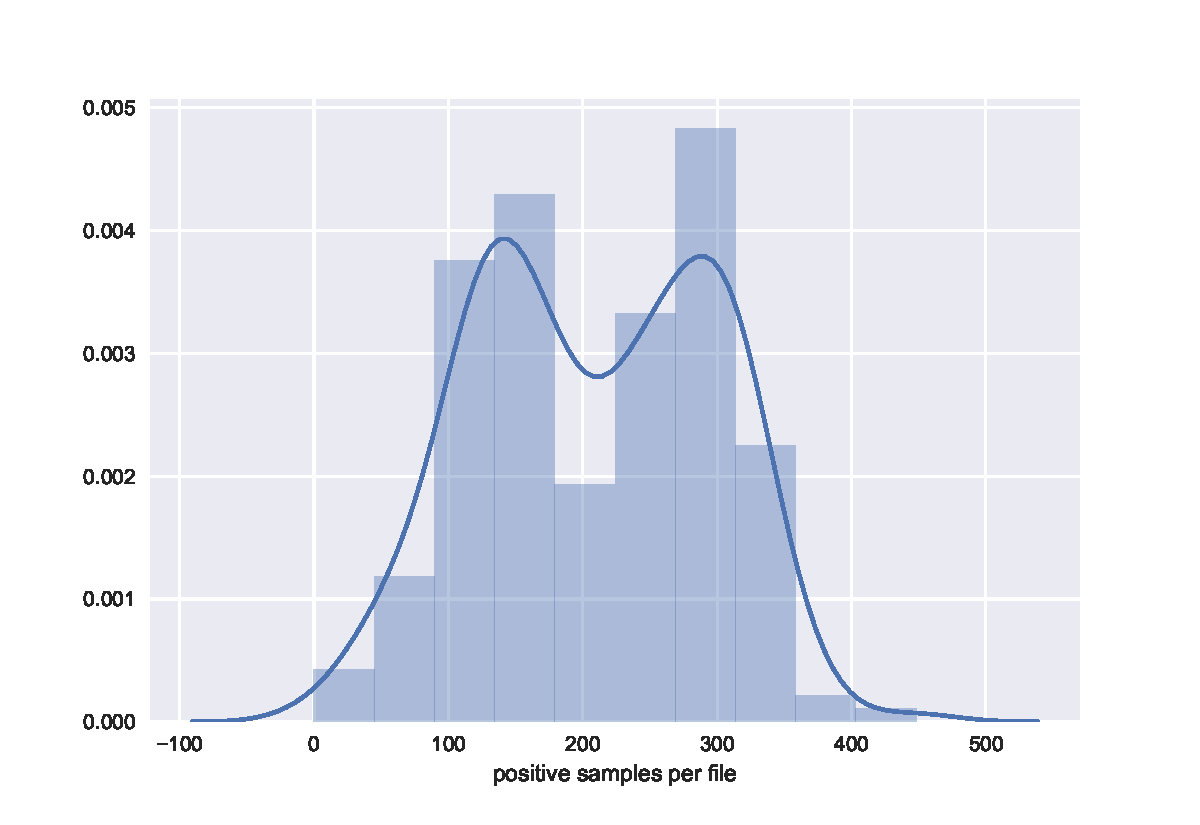
\includegraphics[width=\textwidth]{figures/distribution.pdf}
  \caption{Distribution of the number of positive samples per file}
  \label{fig:data_dist}
\end{figure}

\section{Research Question}
As stated in the introduction, the research done in this thesis is about
augmenting the data with the spatial information that is usually left out in
sentence classification. In doing so, the following research questions will be
considered:
\begin{enumerate}
\item Does this increase the learning performance?
\item Does this allow for reaching the same performance using less data?
\item Does this make the training converge to the optimal performance quicker?
\end{enumerate}

%%% Local Variables:
%%% mode: latex
%%% TeX-master: "report"
%%% End: